\section{CHƯƠNG 2: MẠNG NƠ-RON TÍCH CHẬP (CNN - DEEP VISION)}

\subsection{Tổng quan về Mạng Nơ-ron Tích chập (CNN)}
Mạng Nơ-ron Tích chập (Convolutional Neural Networks - CNN) là một bước đột phá trong lĩnh vực Thị giác máy tính. Khác với các mạng nơ-ron truyền thống, CNN có khả năng tự động trích xuất các đặc trưng không gian (spatial features) từ hình ảnh thông qua các lớp tích chập (Convolution) và lớp gộp (Pooling).

\subsection{Lịch sử và các kiến trúc kinh điển}
Lịch sử của CNN bắt đầu từ LeNet-5 (1998) của Yann LeCun, tiếp nối bởi sự bùng nổ của AlexNet (2012), VGG, ResNet (2015) và gần đây là các mô hình tối ưu như MobileNet và EfficientNet.

\subsection{Kỹ thuật Học chuyển đổi (Transfer Learning)}
Học chuyển đổi là quá trình sử dụng một mô hình đã được huấn luyện trên một tập dữ liệu khổng lồ (như ImageNet) và tinh chỉnh nó cho một bài toán cụ thể khác. Kỹ thuật này giúp tiết kiệm thời gian huấn luyện và tài nguyên tính toán trong khi vẫn đạt được độ chính xác cao.

\subsection{Thực nghiệm chuyên sâu trên 4 Datasets & 4 Models}

\subsubsection{Dataset 1: Intel Image Classification (Custom CNN)}
\textbf{Kiến trúc:} Xây dựng mạng CNN từ đầu với 3 lớp Convolution/Pooling.
\textbf{Mục tiêu:} Hiểu rõ cơ chế hoạt động của từng lớp và cách trích xuất đặc trưng cơ bản từ ảnh phong cảnh.
\paragraph{Thực nghiệm với Intel Image Classification} \hfill \\
Bộ dữ liệu gồm hàng ngàn hình ảnh thuộc 6 lớp phong cảnh: buildings, forest, glacier, mountain, sea, và street.

\paragraph{Mô hình Custom CNN} \hfill \\
Chúng ta thiết kế một mạng CNN đơn giản gồm 3 lớp tích chập với số lượng filter tăng dần (32, 64, 128). Mỗi lớp tích chập đi kèm với lớp ReLU activation và lớp Max Pooling để giảm kích thước đặc trưng.

\paragraph{Kết quả huấn luyện} \hfill \\
\begin{figure}[H]
    \centering
    \includegraphics[width=0.8\linewidth]{Chương_2/results/intel/training_history.png}
    \caption{Lịch sử huấn luyện (Accuracy và Loss) của mạng Custom CNN}
    \label{fig:intel_history}
\end{figure}

Dù kiến trúc đơn giản, mô hình vẫn đạt được độ chính xác khả quan trên tập kiểm tra, chứng minh hiệu quả của việc trích xuất đặc trưng tự động.


\subsubsection{Dataset 2: Flowers-102 (MobileNetV2 - Transfer Learning)}
\textbf{Kiến trúc:} MobileNetV2 (Pre-trained on ImageNet).
\textbf{Mục tiêu:} Áp dụng mô hình nhẹ (lightweight) cho thiết bị di động để phân loại các loài hoa với độ chính xác cao.
\paragraph{Thực nghiệm với Flowers-102} \hfill \\
Bộ dữ liệu chứa hình ảnh của các loài hoa phổ biến. Thách thức của bài toán này nằm ở sự tương đồng về màu sắc và cấu trúc giữa các loài hoa khác nhau.

\paragraph{Phân tích Dữ liệu và Tiền xử lý} \hfill \\
Việc quan sát sự phân bổ dữ liệu cho thấy một số loài hoa có số lượng ảnh áp đảo, điều này đòi hỏi mô hình phải có khả năng học đặc trưng tốt để không bị overfit vào các lớp phổ biến.

\begin{figure}[H]
    \centering
    \begin{minipage}{0.48\textwidth}
        \centering
        
\includegraphics[width=\linewidth]{Chương_2/results/flowers/01_class_distribution.png}
        \caption{Phân bổ dữ liệu các loài hoa}
        \label{fig:flowers_dist}
    \end{minipage}
    \hfill
    \begin{minipage}{0.48\textwidth}
        \centering
        
\includegraphics[width=\linewidth]{Chương_2/results/flowers/02_sample_images.png}
        \caption{Hình ảnh mẫu từ Flowers-102}
        \label{fig:flowers_samples}
    \end{minipage}
\end{figure}

\paragraph{MobileNetV2 và Transfer Learning} \hfill \\
Chúng ta sử dụng MobileNetV2 - một kiến trúc sử dụng tích chập tách biệt theo chiều sâu (Depthwise Separable Convolutions). Mô hình chỉ có \textbf{2,592,325} tham số, cực kỳ nhẹ nhưng vẫn mang lại hiệu suất mạnh mẽ. Bằng cách sử dụng Transfer Learning từ ImageNet, mô hình đã thừa hưởng khả năng nhận diện các hình khối và màu sắc cơ bản.

\paragraph{Kết quả thực nghiệm} \hfill \\
Mô hình đạt độ chính xác ấn tượng là \textbf{86.51\%} trên tập kiểm tra.

\begin{figure}[H]
    \centering
    \begin{minipage}{0.48\textwidth}
        \centering
        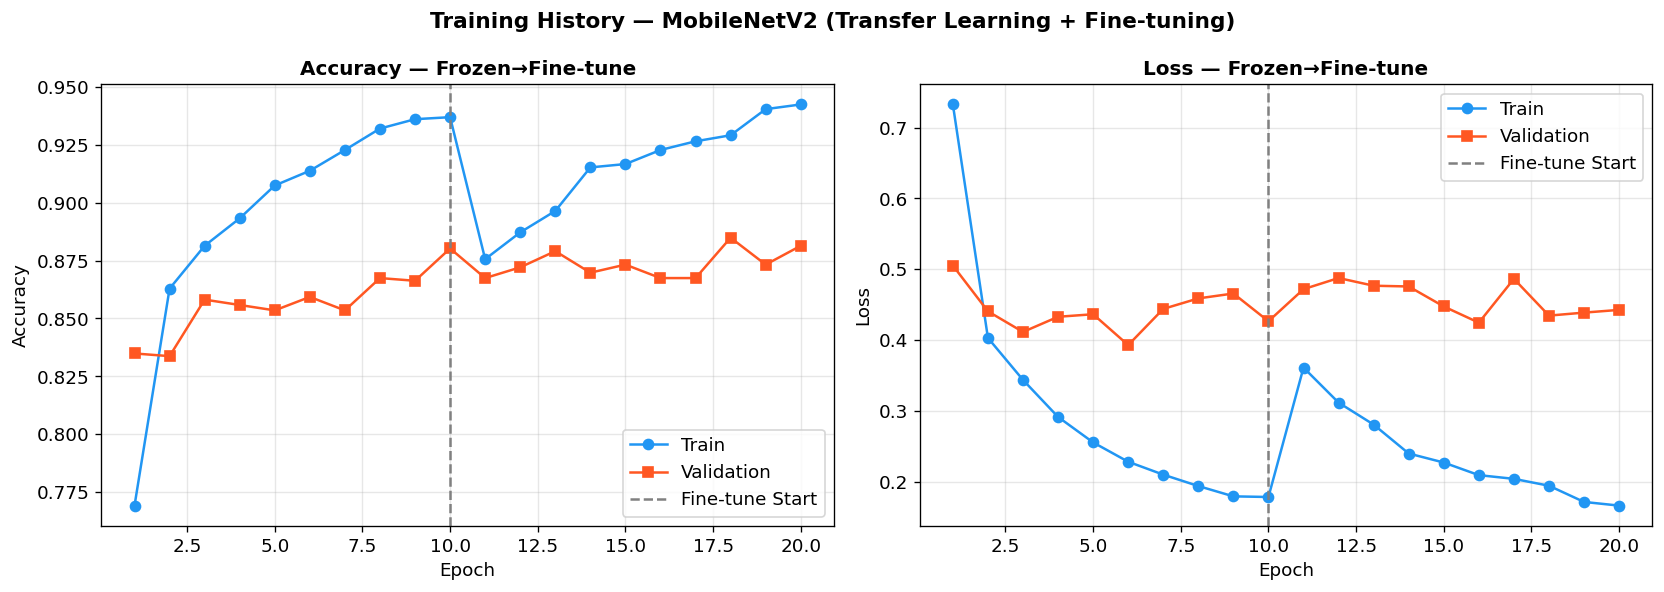
\includegraphics[width=\linewidth]{Chương_2/results/flowers/03_training_history.png}
        \caption{Lịch sử huấn luyện MobileNetV2}
        \label{fig:flowers_history}
    \end{minipage}
    \hfill
    \begin{minipage}{0.48\textwidth}
        \centering
        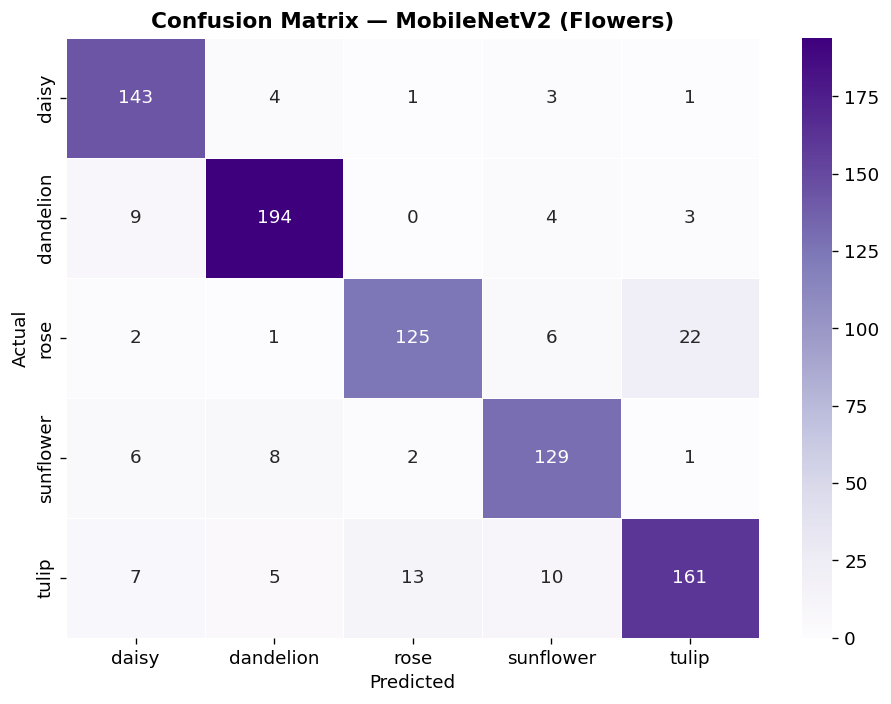
\includegraphics[width=\linewidth]{Chương_2/results/flowers/04_confusion_matrix.png}
        \caption{Ma trận nhầm lẫn phân loại hoa}
        \label{fig:flowers_cm}
    \end{minipage}
\end{figure}

Sử dụng Transfer Learning giúp mô hình không chỉ đạt độ chính xác cao mà còn hội tụ rất nhanh (chỉ sau khoảng 10-15 epoch), tiết kiệm đáng kể tài nguyên tính toán.


\subsubsection{Dataset 3: Chest X-Ray Pneumonia (ResNet-50 - Fine-tuning)}
\textbf{Kiến trúc:} ResNet-50.
\textbf{Mục tiêu:} Ứng dụng AI trong y tế để chẩn đoán viêm phổi từ ảnh X-quang. Sử dụng kiến trúc ResNet với cơ chế Residual blocks để giải quyết vấn đề tiêu biến đạo hàm.
\paragraph{Thực nghiệm với Chest X-Ray Pneumonia} \hfill \\
Đây là bài toán phân loại nhị phân (Binary Classification) có ý nghĩa thực tiễn cao trong y tế. Mục tiêu là phát hiện dấu hiệu viêm phổi qua ảnh chụp X-quang lồng ngực.

\paragraph{Phân tích Dữ liệu Y tế} \hfill \\
Dữ liệu ảnh X-quang thường có độ tương phản thấp và đòi hỏi sự tỉ mỉ trong việc quan sát các vùng mờ.

\begin{figure}[H]
    \centering
    \includegraphics[width=0.8\linewidth]{Chương_2/results/chest_xray/01_dataset_overview.png}
    \caption{Tổng quan dữ liệu ảnh X-quang (Bình thường vs Viêm phổi)}
    \label{fig:chest_overview}
\end{figure}

\paragraph{ResNet-50 và Fine-tuning} \hfill \\
Kiến trúc ResNet-50 với 50 lớp sâu và các kết nối tắt giúp mô hình học được các đặc trưng phức tạp trong ảnh y tế. Với \textbf{24,113,537} tham số, mô hình đủ mạnh để phân biệt các tổn thương mờ nhạt trên phổi.

\paragraph{Kết quả và Phân tích chuyên sâu} \hfill \\
Mô hình đạt chỉ số \textbf{ROC-AUC là 0.9265}. Đặc biệt, trong y tế, chỉ số \textbf{Recall} (độ nhạy) cho lớp \textit{PNEUMONIA} đạt tới \textbf{0.97}, nghĩa là mô hình hầu như không bỏ sót bệnh nhân nào bị viêm phổi.

\begin{figure}[H]
    \centering
    \begin{minipage}{0.48\textwidth}
        \centering
        \includegraphics[width=\linewidth]{Chương_2/results/chest_xray/02_training_history.png}
        \caption{Lịch sử huấn luyện ResNet-50}
        \label{fig:chest_history}
    \end{minipage}
    \hfill
    \begin{minipage}{0.48\textwidth}
        \centering
        \includegraphics[width=\linewidth]{Chương_2/results/chest_xray/03_confusion_roc.png}
        \caption{Confusion Matrix và Đường cong ROC}
        \label{fig:chest_roc}
    \end{minipage}
\end{figure}

Việc ưu tiên Recall giúp hệ thống trở thành một công cụ hỗ trợ đắc lực cho các bác sĩ trong việc sàng lọc ban đầu, giảm thiểu rủi ro chẩn đoán sót.

\paragraph{Phụ lục: Quy trình thực nghiệm chi tiết} \hfill \\
Dưới đây là các bước triển khai chi tiết trên môi trường Jupyter Notebook:

\begin{figure}[H]
    \centering
    
\includegraphics[width=0.9\linewidth]{Chương_2/docs/ch2/17.png}
    \caption{Thiết lập môi trường Y tế: Import kiến trúc ResNet50 và các thư viện xử lý ảnh chuyên sâu.}
\end{figure}

\begin{figure}[H]
    \centering
    
\includegraphics[width=0.9\linewidth]{Chương_2/docs/ch2/18.png}
    \caption{Phân tích độ mất cân bằng lớp: Nhận diện sự chênh lệch lớn giữa lớp Pneumonia (74.3\%) và Normal (25.7\%).}
\end{figure}

\begin{figure}[H]
    \centering
    
\includegraphics[width=0.9\linewidth]{Chương_2/docs/ch2/19.png}
    \caption{Mã nguồn EDA dữ liệu y tế: Vẽ biểu đồ phân bổ lớp kèm theo hiển thị ảnh mẫu cho từng loại.}
\end{figure}

\begin{figure}[H]
    \centering
    
\includegraphics[width=0.9\linewidth]{Chương_2/docs/ch2/20.png}
    \caption{Kết quả Dataset Overview: Hình ảnh so sánh sự khác biệt mờ đục giữa phổi bình thường và phổi bị viêm.}
\end{figure}

\begin{figure}[H]
    \centering
    
\includegraphics[width=0.9\linewidth]{Chương_2/docs/ch2/21.png}
    \caption{Xử lý mất cân bằng: Mã nguồn tính toán `class\_weights` để gán trọng số cao hơn cho lớp thiểu số (Normal).}
\end{figure}

\begin{figure}[H]
    \centering
    
\includegraphics[width=0.9\linewidth]{Chương_2/docs/ch2/22.png}
    \caption{Thiết kế mô hình Transfer Learning: Sử dụng ResNet50 làm Base model và thêm các lớp Dense tùy chỉnh.}
\end{figure}

\begin{figure}[H]
    \centering
    
\includegraphics[width=0.9\linewidth]{Chương_2/docs/ch2/23.png}
    \caption{Quá trình huấn luyện với Trọng số lớp: Sử dụng tham số `class\_weight` trong hàm `fit` để cân bằng mô hình.}
\end{figure}

\begin{figure}[H]
    \centering
    
\includegraphics[width=0.9\linewidth]{Chương_2/docs/ch2/24.png}
    \caption{Mã nguồn trực quan hóa kết quả: Vẽ biểu đồ Accuracy, Loss và đặc biệt là ROC-AUC.}
\end{figure}

\begin{figure}[H]
    \centering
    
\includegraphics[width=0.9\linewidth]{Chương_2/docs/ch2/25.png}
    \caption{Kết quả Training History: Chỉ số ROC-AUC đạt mức ổn định cao (0.92+), chứng minh khả năng phân loại tốt.}
\end{figure}

\begin{figure}[H]
    \centering
    
\includegraphics[width=0.9\linewidth]{Chương_2/docs/ch2/26.png}
    \caption{Mã nguồn đánh giá y tế chuyên sâu: Tính toán Precision, Recall và vẽ đường cong ROC.}
\end{figure}

\begin{figure}[H]
    \centering
    
\includegraphics[width=0.9\linewidth]{Chương_2/docs/ch2/27.png}
    \caption{Kết quả đánh giá cuối cùng: Sự kết hợp giữa Confusion Matrix và ROC Curve cho cái nhìn toàn diện về mô hình.}
\end{figure}


\subsubsection{Dataset 4: Natural Images (EfficientNet-B0 & Grad-CAM)}
\textbf{Kiến trúc:} EfficientNet-B0.
\textbf{Mục tiêu:} Sử dụng mô hình có hiệu năng tối ưu và triển khai Grad-CAM (Gradient-weighted Class Activation Mapping) để trực quan hóa "vùng nhìn" của mô hình, giúp AI trở nên dễ giải thích hơn (Explainable AI).
\paragraph{Thực nghiệm với Natural Images và Grad-CAM} \hfill \\
Bộ dữ liệu gồm 8 lớp đối tượng tự nhiên đa dạng: máy bay, ô tô, mèo, chó, hoa, trái cây, xe máy và người. Đây là thử thách về khả năng tổng quát hóa của mô hình trên các đối tượng có hình thái hoàn toàn khác biệt.

\paragraph{Phân tích Dữ liệu và Tiền xử lý} \hfill \\
Dữ liệu được chia thành 8 lớp với sự đa dạng về góc chụp và bối cảnh.

\begin{figure}[H]
    \centering
    \begin{minipage}{0.48\textwidth}
        \centering
        
\includegraphics[width=\linewidth]{Chương_2/results/natural_images/01_class_distribution.png}
        \caption{Phân bổ dữ liệu 8 lớp đối tượng}
        \label{fig:natural_dist}
    \end{minipage}
    \hfill
    \begin{minipage}{0.48\textwidth}
        \centering
        
\includegraphics[width=\linewidth]{Chương_2/results/natural_images/02_sample_images.png}
        \caption{Hình ảnh mẫu từ bộ dữ liệu Natural Images}
        \label{fig:natural_samples}
    \end{minipage}
\end{figure}

Kỹ thuật Augmentation được áp dụng mạnh mẽ để mô hình không bị phụ thuộc vào vị trí của đối tượng trong khung hình.

\begin{figure}[H]
    \centering
    \includegraphics[width=0.8\linewidth]{Chương_2/results/natural_images/train_batch_visualization.png}
    \caption{Trực quan hóa một batch dữ liệu huấn luyện sau khi qua tiền xử lý}
    \label{fig:natural_batch}
\end{figure}

\paragraph{EfficientNet-B0} \hfill \\
EfficientNet sử dụng kỹ thuật Compound Scaling để cân bằng giữa độ sâu, độ rộng và độ phân giải của mạng. Với chỉ \textbf{4,384,683} tham số, mô hình đạt được hiệu năng vượt trội so với nhiều kiến trúc nặng hơn.

\paragraph{Kết quả huấn luyện và Trực quan hóa Grad-CAM} \hfill \\
Mô hình đạt độ chính xác \textbf{72\%} trên tập kiểm tra. Để giải thích quyết định của mô hình, chúng ta sử dụng kỹ thuật Grad-CAM.

\begin{figure}[H]
    \centering
    \begin{minipage}{0.48\textwidth}
        \centering
        
\includegraphics[width=\linewidth]{Chương_2/results/natural_images/03_training_history.png}
        \caption{Lịch sử huấn luyện EfficientNet}
        \label{fig:natural_history}
    \end{minipage}
    \hfill
    \begin{minipage}{0.48\textwidth}
        \centering
        
\includegraphics[width=\linewidth]{Chương_2/results/natural_images/04_confusion_matrix.png}
        \caption{Ma trận nhầm lẫn đa lớp}
        \label{fig:natural_cm}
    \end{minipage}
\end{figure}

\begin{figure}[H]
    \centering
    \includegraphics[width=0.8\linewidth]{Chương_2/results/natural_images/05_gradcam_visualization.png}
    \caption{Trực quan hóa Grad-CAM: Giải thích "vùng nhìn" của AI cho từng lớp đối tượng}
    \label{fig:gradcam}
\end{figure}

Biểu đồ Grad-CAM cho thấy mô hình đã tập trung đúng vào các đặc trưng quan trọng của đối tượng (ví dụ: tập trung vào phần thân và bánh xe của ô tô, khuôn mặt của mèo/chó). Điều này khẳng định mô hình không chỉ đạt độ chính xác tốt mà còn học được các đặc trưng ngữ nghĩa đúng đắn.


\subsection{Tổng kết Chương 2}
Thông qua 4 thực nghiệm, chúng ta thấy được sự tiến hóa từ việc xây dựng model thủ công đến việc tận dụng sức mạnh của Transfer Learning. Đặc biệt, việc kết hợp Grad-CAM giúp tăng tính tin cậy của AI trong các ứng dụng thực tế.
